%&pdflatex
%% filename: amsart-template.tex, version: 2.1
\documentclass{amsart}
\usepackage{hyperref}
\usepackage{inputenc}
\usepackage{graphicx}
\usepackage{bbm}

\newtheorem{theorem}{Theorem}[section]
\newtheorem{lemma}[theorem]{Lemma}
\theoremstyle{definition}
\newtheorem{definition}[theorem]{Definition}
\newtheorem{example}[theorem]{Example}
\newtheorem{xca}[theorem]{Exercise}
\theoremstyle{remark}
\newtheorem{remark}[theorem]{Remark}
\numberwithin{equation}{section}
\setlength{\parindent}{0pt} % turn off auto-indent

\graphicspath{ {./} }

\begin{document}

\title{Assignment 3: Neural Turing Machines [IFT6135]}

\author{Joseph D. Viviano, Marzi Mehdizad, Johnathan Guymont}
\address{Universit\'e de Montr\'eal}
\curraddr{}
\email{joseph@viviano.ca, jonathan@guymont.com, marzieh.mehdizadeh@gmail.com}
\thanks{}
\date{March 2018}

\maketitle

\section{Implementing the Neural Turing Machine}

Our implementation was forked from \url{https://github.com/loudinthecloud/pytorch-ntm}.
The code can be found at \url{https://github.com/josephdviviano/pytorch-ntm}.\\

\subsection{Parameters}

As requested, all models made use of a single 100-node layer (for the NTM models,
this layer was in the controller, for the LSTM, this layer was the hidden layer).
Both NTM models used a single read and write head.


\begin{enumerate}
  \item{LSTM-NTM: number of parameters = 62860}
  \item{MLP-NTM: number of parameters = 13260}
  \item{LSTM (baseline): number of parameters = 45408}
\end{enumerate}

\subsection{Hyperparameters Chosen}

The same hyperparameters were used for all models to facilitate comparison. All
models were trained on 40000 sequences, with a random length between 1 and 20.
We used the rmsprop optimizer, with a learning rate of 0.0004, momentum of 0.9,
and alpha of 0.95. The loss was binary cross entropy. \\

Please see figure 1-3 for the convergence of the three models (LSTM-NTM,
MLP-NTM, and LSTM baseline) using these hyperparameters, respectively. \\

\begin{figure}[h]
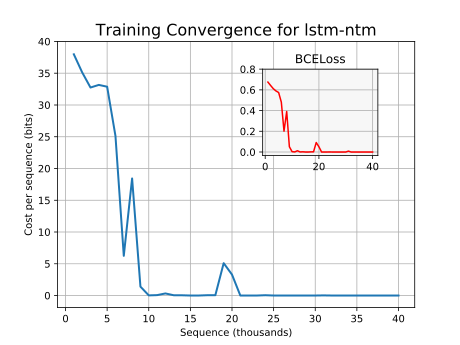
\includegraphics[width=100mm]{outputs/lstm-ntm_convergence}
\caption{Training curve of LSTM-NTM.}
\label{Figure 1}
\end{figure}

\begin{figure}[h]
\includegraphics[width=100mm]{outputs/mlp-ntm_convergence}
\caption{Training curve of MLP-NTM.}
\label{Figure 2}
\end{figure}

\begin{figure}[h]
\includegraphics[width=100mm]{outputs/lstm_convergence}
\caption{Training curve of LSTM baseline.}
\label{Figure 3}
\end{figure}

Furthermore, the curve per sequence size can be seen for each in figures 4-6:\\

\begin{figure}[h]
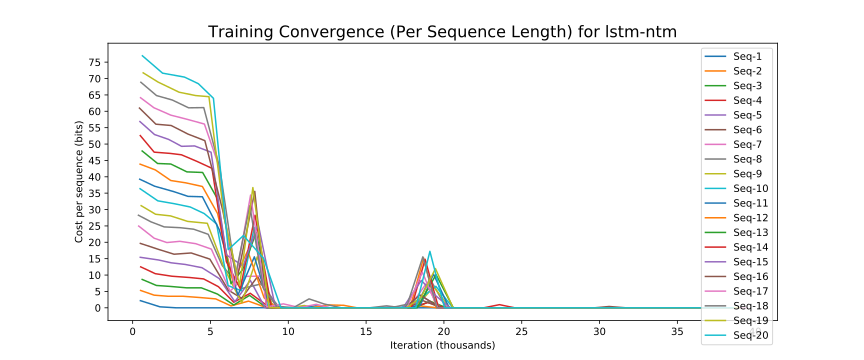
\includegraphics[width=100mm]{outputs/lstm-ntm_convergence-perlen}
\caption{Length-specific training curves of the LSTM-NTM.}
\label{Figure 4}
\end{figure}

\begin{figure}[h]
\includegraphics[width=100mm]{outputs/mlp-ntm_convergence-perlen}
\caption{Length-specific training curves of the MLP-NTM.}
\label{Figure 5}
\end{figure}

\begin{figure}[h]
\includegraphics[width=100mm]{outputs/lstm_convergence-perlen}
\caption{Length-specific training curves of the LSTM baseline.}
\label{Figure 6}
\end{figure}

It can be seen that the LSTM-NTM model converges fastest, followed by the
MLP-NTM. The LSTM model improves over time, but does not converge nearly as
quickly as either NTM model, replicating the `qualitative' difference between
methods noted in the original paper. \\

\subsection{Generalization to Longer Sequences}



\subsection{Visualization of Read/Write Heads (Attention)}
\subsection{Understanding the Shift Operator}

\end{document}

